\chapter{Analysis and Specification of Requirements}

\section*{Introduction}
This chapter presents a comprehensive analysis and specification of requirements for the MindCare-IA platform, a sophisticated Django-based mental health application designed to facilitate interaction between therapists and patients. The meticulous identification and documentation of both functional and non-functional requirements are pivotal to ensuring the final system effectively addresses the complex needs of mental healthcare delivery while meeting stakeholders' expectations.

The requirements engineering process employed multiple methodologies to gather complete and accurate specifications:
\begin{itemize}
    \item \textbf{Domain Analysis:} Examination of existing mental health platforms and healthcare systems to identify industry standards and best practices
    \item \textbf{Stakeholder Interviews:} Structured consultations with mental health professionals and potential users to capture diverse perspectives
    \item \textbf{Technical Feasibility Assessment:} Evaluation of modern technologies including Django's capabilities for implementing secure and scalable solutions
    \item \textbf{Regulatory Compliance Research:} Investigation of healthcare data protection regulations and privacy standards
\end{itemize}

MindCare-IA aims to revolutionize mental healthcare delivery through a feature-rich platform integrating secure messaging, appointment scheduling, therapy session management, mood tracking, and therapeutic interventions. The system architecture leverages Django's robust framework to implement microservices for user management, real-time communication, notification delivery, and data analytics while maintaining strict security protocols.

The requirements documented in this chapter serve three essential purposes:
\begin{enumerate}
    \item Provide a clear roadmap for the development team to implement features and functionalities
    \item Establish measurable criteria for system validation and acceptance testing
    \item Create a shared understanding among stakeholders about the scope and capabilities of the final system
\end{enumerate}

\section{Analysis and Specification of Functional Requirements}
Functional requirements describe what the system should do, specifying the features and functionalities that must be implemented. These requirements define the core capabilities of the system and outline the behaviors it should exhibit under specific conditions.

\subsection{Identification of Actors}
This section identifies the primary actors who interact with the MindCare-IA system. An actor represents a role that a user or external system plays when interacting with the application.

\begin{table}[h]
\centering
\begin{tabular}{|p{3cm}|p{10cm}|}
\hline
\textbf{Actor} & \textbf{Description} \\
\hline
Patient & End user seeking mental health support. Patients can schedule appointments, communicate with therapists, track their mood, maintain a personal journal, and interact with the AI chatbot. \\
\hline
Therapist & Mental health professional providing care. Therapists manage patient relationships, conduct therapy sessions, view patient mood data, maintain session notes, and manage their availability calendar. \\
\hline
System Administrator & Technical user responsible for system maintenance, therapist verification, and platform configuration. \\
\hline
AI Chatbot & Autonomous component providing immediate mental health support through natural language processing capabilities. \\
\hline
External Authentication Provider & Third-party identity provider (Google) that handles user authentication via OAuth 2.0. \\
\hline
Notification System & Internal component responsible for delivering real-time messages and alerts to users across different channels (in-app, email). \\
\hline
\end{tabular}
\caption{Primary Actors in the MindCare-IA System}
\end{table}

\subsubsection{Actor Relationships and Interactions}
The following describes the key relationships between different actors and how they interact with the system:

\begin{itemize}
    \item \textbf{Patient-Therapist Relationship:} A core relationship where patients connect with therapists for mental health services. This is facilitated through messaging, appointments, and mood tracking features.
    
    \item \textbf{Patient-Chatbot Interaction:} Supplementary support mechanism where patients can receive immediate assistance from an AI-powered system when human therapists are unavailable.
    
    \item \textbf{Therapist-Administrator Interaction:} Administrative workflow where therapists submit credentials for verification and administrators validate them to ensure professional standards.
    
    \item \textbf{System-User Notification:} System-initiated communication to keep users informed of relevant events, such as new messages, appointment reminders, or status updates.
\end{itemize}

\subsection{Expression of Functional Requirements}
The functional requirements of the MindCare-IA platform have been systematically organized according to the primary system modules identified during the domain analysis. Each requirement follows the format: "The system shall [capability]" to ensure clarity and testability.

\subsubsection{User Management}
\begin{itemize}
    \item The system shall allow users to register with email and password
    \item The system shall implement secure authentication mechanisms including JWT-based token authentication
    \item The system shall support OAuth 2.0 authentication with Google as an external identity provider
    \item The system shall support different user roles (patient, therapist, administrator) with role-specific permissions
    \item The system shall allow users to reset their password through a secure email verification process
    \item The system shall maintain user profiles with personal information and role-specific attributes
    \item The system shall implement email verification for new user registrations to prevent fraudulent accounts
    \item The system shall allow users to manage their notification preferences and privacy settings
\end{itemize}

\subsubsection{Core System Functionality}
\begin{itemize}
    \item The system shall provide comprehensive messaging capabilities including one-to-one conversations between therapists and patients, group conversations for support groups, and an AI-powered chatbot for immediate assistance
    \item The system shall allow therapists to manage appointments with patients including scheduling, rescheduling, and cancellation with appropriate notifications
    \item The system shall support patient mood tracking and journaling functionality to monitor mental health progress over time
    \item The system shall enable therapists to create and maintain session notes documenting patient interactions and progress
    \item The system shall implement a notification system to alert users of important events such as new messages, appointment reminders, and system updates
    \item The system shall provide therapist verification processes to ensure credentials are valid before allowing patient interactions
    \item The system shall support real-time communication features such as typing indicators and online presence detection
    \item The system shall enable secure file sharing between patients and therapists for relevant documentation
\end{itemize}

\subsubsection{Data Management}
\begin{itemize}
    \item The system shall store and manage user profiles including patient and therapist-specific data with appropriate access controls
    \item The system shall maintain healthcare records including medical history, mood logs, and therapy session notes with strict privacy protections
    \item The system shall track appointment data including scheduling, history, and outcomes to facilitate continuity of care
    \item The system shall store messaging content (individual, group, and chatbot conversations) with appropriate encryption and retention policies
    \item The system shall manage media uploads including profile pictures, verification documents, and shared files with proper validation and security measures
    \item The system shall implement comprehensive data validation rules for all input, including therapist credentials and patient health information
    \item The system shall ensure data integrity through transaction management and consistency checks across all database operations
    \item The system shall provide secure backup and recovery mechanisms for all healthcare data in compliance with relevant regulations
\end{itemize}

\section{General Use Case Diagram}

A use case diagram provides a visual representation of the interactions between actors and the system. The diagram below illustrates the primary use cases of the MindCare-IA mental health platform, depicting how the various actors identified in the previous section interact with the system functionalities.

\begin{figure}[h]
\centering
% Include this code if you have an external image file for the diagram
% \includegraphics[width=0.9\textwidth]{figures/use_case_diagram.png}

% Alternatively, create the diagram directly with TikZ
\begin{tikzpicture}[scale=0.7]
% Define styles for actors and use cases
\tikzstyle{actor}=[draw, rounded corners, fill=gray!20, text width=2.5cm, minimum height=1cm, align=center]
\tikzstyle{usecase}=[draw, ellipse, fill=blue!20, text width=3cm, align=center]
\tikzstyle{system}=[draw, rectangle, dashed, align=center, text width=14cm]

% Define system boundary
\node[system] (system) at (5, 0) {\textbf{MindCare-IA Platform}};
\draw (system.north west) -- (system.north east);
\node[align=center] at (5, 11) {\textbf{MindCare-IA Platform}};

% Define actors
\node[actor] (patient) at (-4, 8) {Patient};
\node[actor] (therapist) at (-4, 0) {Therapist};
\node[actor] (admin) at (-4, -8) {System Administrator};
\node[actor] (chatbot) at (14, 4) {AI Chatbot};
\node[actor] (auth) at (14, -4) {External Authentication Provider};

% Define use cases
\node[usecase] (register) at (0, 10) {Register/Login};
\node[usecase] (manage_profile) at (3, 8) {Manage Profile};
\node[usecase] (messaging) at (5, 6) {Send/Receive Messages};
\node[usecase] (mood_tracking) at (9, 10) {Track Mood};
\node[usecase] (journaling) at (9, 8) {Maintain Journal};

\node[usecase] (appointments) at (3, 2) {Manage Appointments};
\node[usecase] (session_notes) at (7, 0) {Create Session Notes};
\node[usecase] (verify) at (7, -2) {Complete Verification};
\node[usecase] (view_metrics) at (5, -4) {View Patient Metrics};

\node[usecase] (verify_therapists) at (3, -8) {Verify Therapists};
\node[usecase] (system_config) at (7, -8) {Configure System};

\node[usecase] (ai_support) at (10, 4) {Provide AI Support};
\node[usecase] (oauth) at (10, -6) {Authentication via OAuth};

% Define relationships
\draw (patient) -- (register);
\draw (patient) -- (manage_profile);
\draw (patient) -- (messaging);
\draw (patient) -- (mood_tracking);
\draw (patient) -- (journaling);
\draw (patient) -- (appointments);

\draw (therapist) -- (register);
\draw (therapist) -- (manage_profile);
\draw (therapist) -- (messaging);
\draw (therapist) -- (appointments);
\draw (therapist) -- (session_notes);
\draw (therapist) -- (verify);
\draw (therapist) -- (view_metrics);

\draw (admin) -- (verify_therapists);
\draw (admin) -- (system_config);

\draw (chatbot) -- (ai_support);
\draw (auth) -- (oauth);

\draw[dashed, ->] (messaging) -- (ai_support);
\draw[dashed, ->] (register) -- (oauth);

% Include relationship labels if needed
\node[text width=2cm, align=center, font=\small] at (1.5, 5) {participates};

\end{tikzpicture}
\caption{General Use Case Diagram for MindCare-IA Platform}
\label{fig:use_case_diagram}
\end{figure}

\section{Use Cases}

Based on the analysis of the MindCare-IA platform requirements, the following detailed use cases have been identified. These use cases represent the core functionalities of the system and describe how different actors interact with the platform.

\subsection{Use Case 1: Patient-Therapist Communication}
\begin{figure}[h]
\centering
\begin{tikzpicture}
\tikzstyle{actor}=[draw, rounded corners=3pt, fill=gray!20, text width=2cm, minimum height=1cm, align=center]
\tikzstyle{usecase}=[draw, ellipse, fill=blue!20, text width=3.5cm, align=center]
\tikzstyle{system}=[draw, rectangle, dashed, minimum width=12cm, minimum height=8cm]
\tikzstyle{line}=[draw]
\tikzstyle{arrow}=[->, >=stealth, thick]

% System boundary
\node[system] (sys) at (4,0) {};
\node[align=center] at (4,4) {\textbf{MindCare-IA: Patient-Therapist Communication}};

% Actors
\node[actor] (patient) at (-2,2) {Patient};
\node[actor] (therapist) at (-2,-2) {Therapist};

% Use Cases
\node[usecase] (message) at (4,3) {Send/Receive Messages};
\node[usecase] (attach) at (4,1) {Share Files/Media};
\node[usecase] (read) at (4,-1) {View Message History};
\node[usecase] (typing) at (4,-3) {See Typing Indicators};

% Connections
\draw[line] (patient) -- (message);
\draw[line] (patient) -- (attach);
\draw[line] (patient) -- (read);
\draw[line] (patient) -- (typing);
\draw[line] (therapist) -- (message);
\draw[line] (therapist) -- (attach);
\draw[line] (therapist) -- (read);
\draw[line] (therapist) -- (typing);
\end{tikzpicture}
\caption{Use Case Diagram: Patient-Therapist Communication}
\end{figure}

\subsubsection{Sequence Diagram for Patient-Therapist Communication}
\begin{figure}[h]
\centering
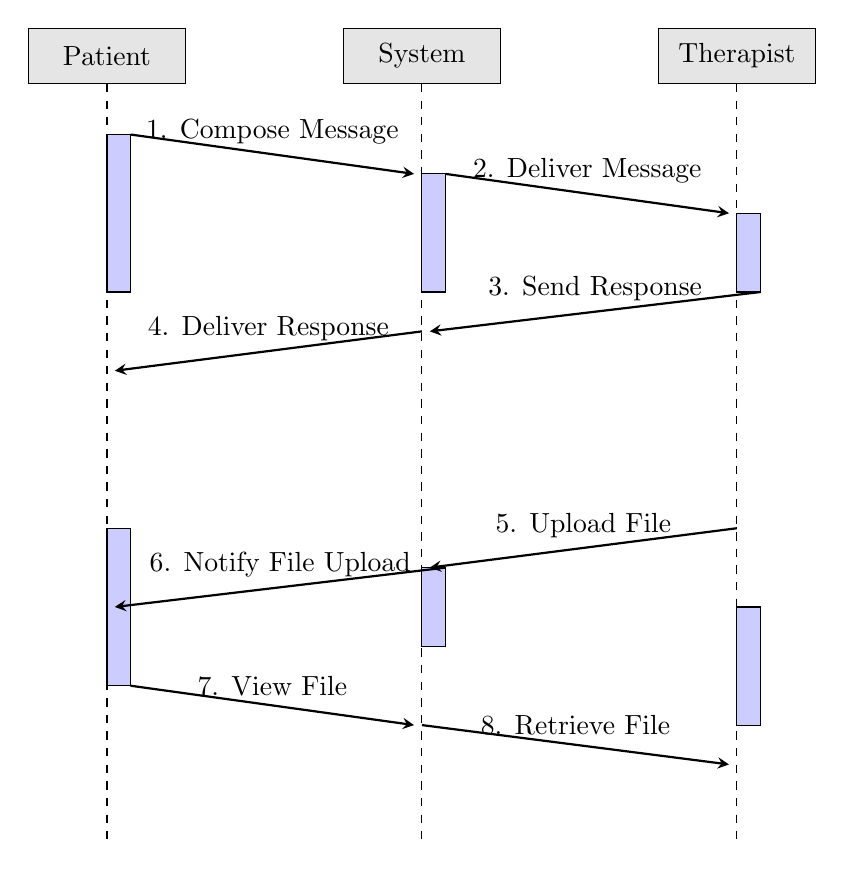
\begin{tikzpicture}
\tikzstyle{actor}=[draw, rectangle, minimum width=2cm, minimum height=0.7cm, fill=gray!20, text centered]
\tikzstyle{line}=[draw, -stealth, thick]
\tikzstyle{lifeline}=[draw, dashed]
\tikzstyle{activation}=[draw, fill=blue!20, minimum width=0.3cm]

% Define actors
\node[actor] (patient) at (0,0) {Patient};
\node[actor] (system) at (4,0) {System};
\node[actor] (therapist) at (8,0) {Therapist};

% Draw lifelines
\draw[lifeline] (patient) -- +(0,-10);
\draw[lifeline] (system) -- +(0,-10);
\draw[lifeline] (therapist) -- +(0,-10);

% Activation boxes
\draw[activation] (0,-1) rectangle +(0.3,-2);
\draw[activation] (4,-1.5) rectangle +(0.3,-1.5);
\draw[activation] (8,-2) rectangle +(0.3,-1);

\draw[activation] (0,-6) rectangle +(0.3,-2);
\draw[activation] (4,-6.5) rectangle +(0.3,-1);
\draw[activation] (8,-7) rectangle +(0.3,-1.5);

% Message flow
\draw[line] (0.3,-1) -- node[above] {1. Compose Message} (3.9,-1.5);
\draw[line] (4.3,-1.5) -- node[above] {2. Deliver Message} (7.9,-2);
\draw[line] (8.3,-3) -- node[above] {3. Send Response} (4.1,-3.5);
\draw[line] (4,-3.5) -- node[above] {4. Deliver Response} (0.1,-4);

\draw[line] (8,-6) -- node[above] {5. Upload File} (4.1,-6.5);
\draw[line] (4.3,-6.5) -- node[above] {6. Notify File Upload} (0.1,-7);
\draw[line] (0.3,-8) -- node[above] {7. View File} (3.9,-8.5);
\draw[line] (4,-8.5) -- node[above] {8. Retrieve File} (7.9,-9);
\end{tikzpicture}
\caption{Sequence Diagram: Patient-Therapist Communication Process}
\end{figure}

\subsubsection{Use Case Description}
\begin{table}[h]
\centering
\begin{tabular}{|p{3cm}|p{10cm}|}
\hline
\textbf{Use Case} & Patient-Therapist Communication \\
\hline
\textbf{Actor} & Patient, Therapist \\
\hline
\textbf{Precondition} & 
\begin{itemize}
    \item Both users are authenticated in the system
    \item Therapist has a verified profile
    \item A therapeutic relationship has been established
\end{itemize} \\
\hline
\textbf{Main Scenario Description} & 
\begin{enumerate}
    \item User initiates or continues a conversation
    \item System displays the messaging interface with conversation history
    \item User composes and sends a message or attachment
    \item System delivers the message with appropriate notifications
    \item Recipient views the message and can respond
    \item System updates conversation with read receipts
    \item Users can exchange files and media related to therapy
    \item System maintains secure record of all communications
\end{enumerate} \\
\hline
\textbf{Postcondition} & 
\begin{itemize}
    \item Messages are securely stored in the system
    \item Both users can view the complete conversation history
    \item Read receipts indicate message delivery status
\end{itemize} \\
\hline
\textbf{Exception} & 
\begin{itemize}
    \item If connectivity is lost, messages are queued for delivery when connection is restored
    \item If user uploads files that exceed size limit, system shows error message
    \item If content violates platform guidelines, system flags for review
\end{itemize} \\
\hline
\end{tabular}
\caption{Use Case Description: Patient-Therapist Communication}
\end{table}

\subsection{Use Case 2: Appointment Management}
\begin{figure}[h]
\centering
\begin{tikzpicture}
\tikzstyle{actor}=[draw, rounded corners=3pt, fill=gray!20, text width=2cm, minimum height=1cm, align=center]
\tikzstyle{usecase}=[draw, ellipse, fill=blue!20, text width=3.5cm, align=center]
\tikzstyle{system}=[draw, rectangle, dashed, minimum width=12cm, minimum height=8cm]
\tikzstyle{line}=[draw]
\tikzstyle{arrow}=[->, >=stealth, thick]

% System boundary
\node[system] (sys) at (4,0) {};
\node[align=center] at (4,4) {\textbf{MindCare-IA: Appointment Management}};

% Actors
\node[actor] (patient) at (-2,2) {Patient};
\node[actor] (therapist) at (-2,-2) {Therapist};
\node[actor] (notif) at (10,0) {Notification System};

% Use Cases
\node[usecase] (schedule) at (4,3) {Schedule Appointment};
\node[usecase] (reschedule) at (4,1) {Reschedule Appointment};
\node[usecase] (cancel) at (4,-1) {Cancel Appointment};
\node[usecase] (remind) at (4,-3) {Receive Reminders};

% Connections
\draw[line] (patient) -- (schedule);
\draw[line] (patient) -- (reschedule);
\draw[line] (patient) -- (cancel);
\draw[line] (patient) -- (remind);
\draw[line] (therapist) -- (schedule);
\draw[line] (therapist) -- (reschedule);
\draw[line] (therapist) -- (cancel);
\draw[line] (therapist) -- (remind);
\draw[arrow, dashed] (remind) -- (notif);
\end{tikzpicture}
\caption{Use Case Diagram: Appointment Management}
\end{figure}

\subsubsection{Sequence Diagram for Appointment Management}
\begin{figure}[h]
\centering
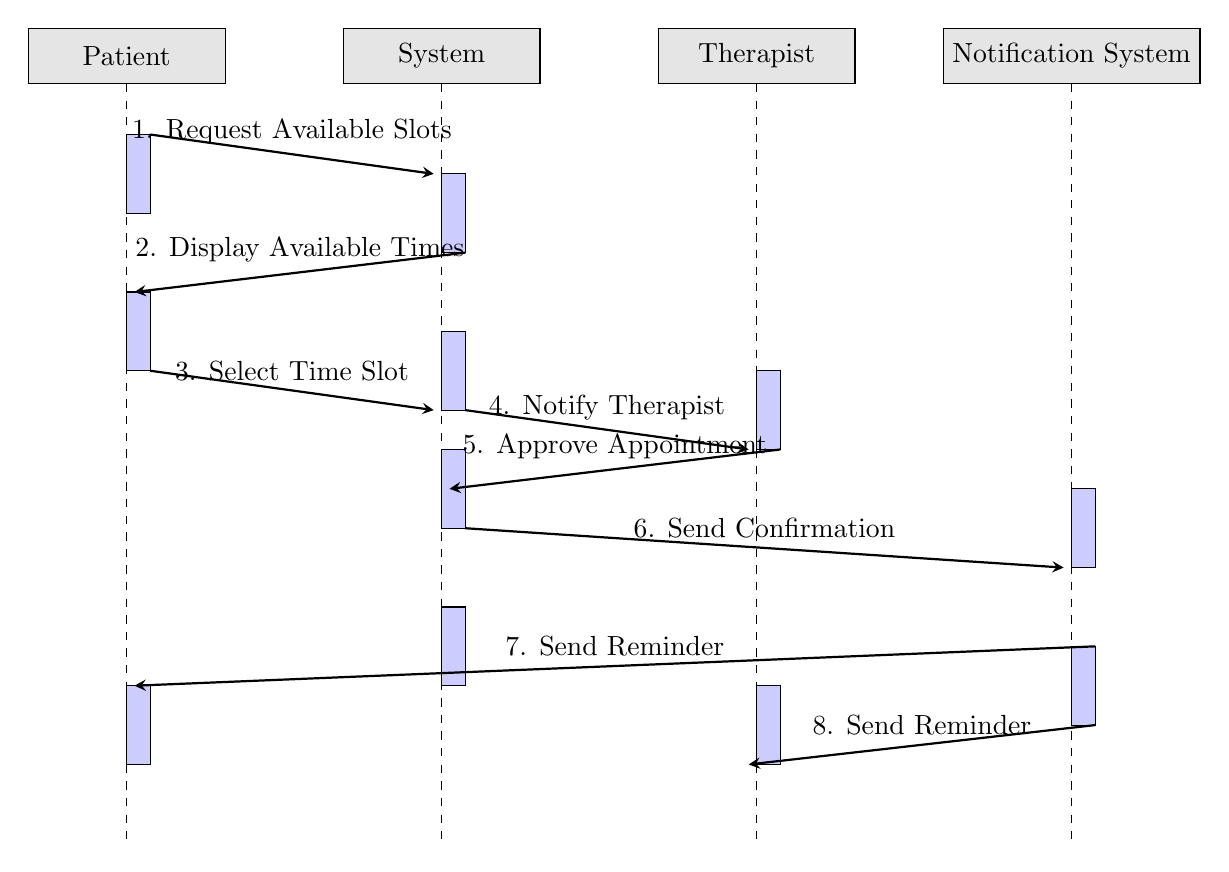
\begin{tikzpicture}
\tikzstyle{actor}=[draw, rectangle, minimum width=2.5cm, minimum height=0.7cm, fill=gray!20, text centered]
\tikzstyle{line}=[draw, -stealth, thick]
\tikzstyle{lifeline}=[draw, dashed]
\tikzstyle{activation}=[draw, fill=blue!20, minimum width=0.3cm]

% Define actors
\node[actor] (patient) at (0,0) {Patient};
\node[actor] (system) at (4,0) {System};
\node[actor] (therapist) at (8,0) {Therapist};
\node[actor] (notif) at (12,0) {Notification System};

% Draw lifelines
\draw[lifeline] (patient) -- +(0,-10);
\draw[lifeline] (system) -- +(0,-10);
\draw[lifeline] (therapist) -- +(0,-10);
\draw[lifeline] (notif) -- +(0,-10);

% Activation boxes
\draw[activation] (0,-1) rectangle +(0.3,-1);
\draw[activation] (4,-1.5) rectangle +(0.3,-1);
\draw[activation] (0,-3) rectangle +(0.3,-1);
\draw[activation] (4,-3.5) rectangle +(0.3,-1);
\draw[activation] (8,-4) rectangle +(0.3,-1);
\draw[activation] (4,-5) rectangle +(0.3,-1);
\draw[activation] (12,-5.5) rectangle +(0.3,-1);
\draw[activation] (4,-7) rectangle +(0.3,-1);
\draw[activation] (12,-7.5) rectangle +(0.3,-1);
\draw[activation] (0,-8) rectangle +(0.3,-1);
\draw[activation] (8,-8) rectangle +(0.3,-1);

% Message flow
\draw[line] (0.3,-1) -- node[above] {1. Request Available Slots} (3.9,-1.5);
\draw[line] (4.3,-2.5) -- node[above] {2. Display Available Times} (0.1,-3);
\draw[line] (0.3,-4) -- node[above] {3. Select Time Slot} (3.9,-4.5);
\draw[line] (4.3,-4.5) -- node[above] {4. Notify Therapist} (7.9,-5);
\draw[line] (8.3,-5) -- node[above] {5. Approve Appointment} (4.1,-5.5);
\draw[line] (4.3,-6) -- node[above] {6. Send Confirmation} (11.9,-6.5);
\draw[line] (12.3,-7.5) -- node[above] {7. Send Reminder} (0.1,-8);
\draw[line] (12.3,-8.5) -- node[above] {8. Send Reminder} (7.9,-9);
\end{tikzpicture}
\caption{Sequence Diagram: Appointment Management Process}
\end{figure}

\subsubsection{Use Case Description}
\begin{table}[h]
\centering
\begin{tabular}{|p{3cm}|p{10cm}|}
\hline
\textbf{Use Case} & Appointment Management \\
\hline
\textbf{Actor} & Patient, Therapist, Notification System \\
\hline
\textbf{Precondition} & 
\begin{itemize}
    \item Therapist has configured availability in their profile
    \item Patient is registered and has access to booking functionality
    \item Patient and therapist have an established therapeutic relationship
\end{itemize} \\
\hline
\textbf{Main Scenario Description} & 
\begin{enumerate}
    \item Patient requests to book an appointment
    \item System displays available time slots based on therapist's calendar
    \item Patient selects preferred date and time
    \item System notifies therapist of the appointment request
    \item Therapist approves the appointment
    \item System sends confirmation notification and updates calendars
    \item System sends reminders as the appointment approaches
    \item Appointment takes place at the scheduled time
\end{enumerate} \\
\hline
\textbf{Postcondition} & 
\begin{itemize}
    \item Appointment is recorded in the system
    \item Event appears on both users' calendars
    \item System schedules automatic reminders
\end{itemize} \\
\hline
\textbf{Exception} & 
\begin{itemize}
    \item If therapist rejects appointment, patient is notified to select alternative time
    \item If appointment needs rescheduling, either party can initiate the change with notifications sent
    \item If appointment is canceled, system frees the time slot and notifies affected parties
\end{itemize} \\
\hline
\end{tabular}
\caption{Use Case Description: Appointment Management}
\end{table}

\subsection{Use Case 5: Mood Tracking}
\begin{figure}[h]
\centering
\begin{tikzpicture}
\tikzstyle{actor}=[draw, rounded corners=3pt, fill=gray!20, text width=2cm, minimum height=1cm, align=center]
\tikzstyle{usecase}=[draw, ellipse, fill=blue!20, text width=3.5cm, align=center]
\tikzstyle{system}=[draw, rectangle, dashed, minimum width=12cm, minimum height=8cm]
\tikzstyle{line}=[draw]
\tikzstyle{extend}=[draw, ->, >=stealth, dashed]

% System boundary
\node[system] (sys) at (4,0) {};
\node[align=center] at (4,4) {\textbf{MindCare-IA: Mood Tracking}};

% Actors
\node[actor] (patient) at (-2,0) {Patient};
\node[actor] (therapist) at (10,0) {Therapist};

% Use Cases
\node[usecase] (record) at (2,2) {Record Daily Mood};
\node[usecase] (notes) at (2,0) {Add Contextual Notes};
\node[usecase] (history) at (2,-2) {View Mood History};
\node[usecase] (analyze) at (6,1) {Generate Mood Analytics};
\node[usecase] (review) at (6,-1) {Review Patient Mood Patterns};

% Connections
\draw[line] (patient) -- (record);
\draw[line] (patient) -- (notes);
\draw[line] (patient) -- (history);
\draw[line] (therapist) -- (review);
\draw[extend] (history) -- (analyze) node[midway, above, sloped, font=\small] {<<includes>>};
\draw[extend] (analyze) -- (review) node[midway, above, sloped, font=\small] {<<extends>>};
\end{tikzpicture}
\caption{Use Case Diagram: Mood Tracking}
\end{figure}

\subsubsection{Sequence Diagram for Mood Tracking}
\begin{figure}[h]
\centering
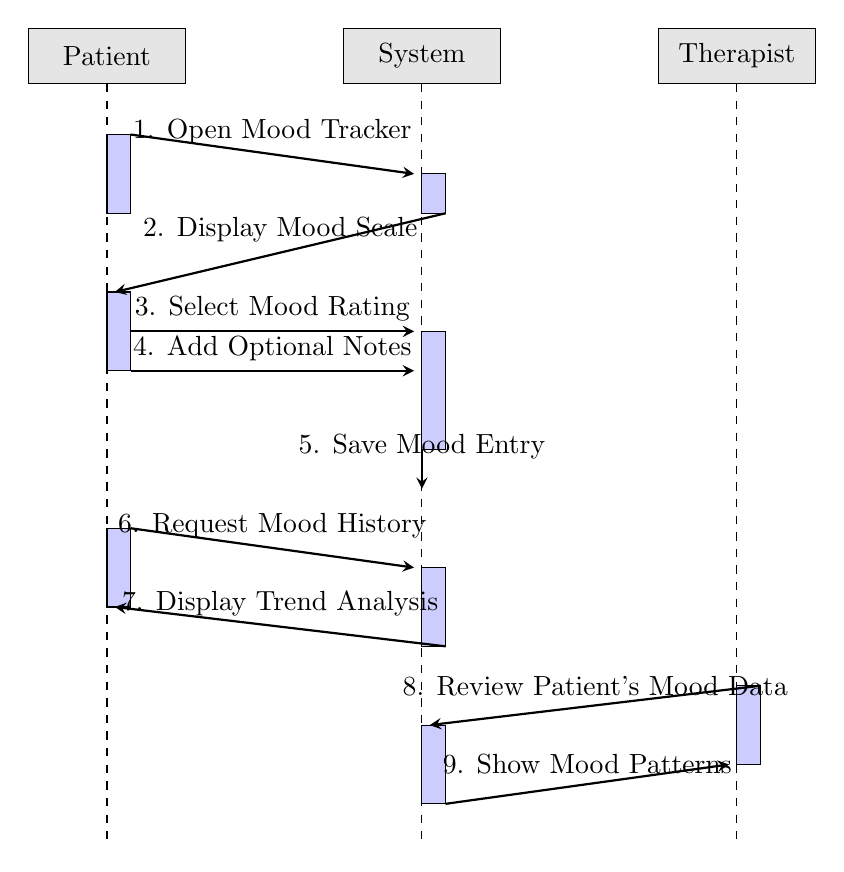
\begin{tikzpicture}
\tikzstyle{actor}=[draw, rectangle, minimum width=2cm, minimum height=0.7cm, fill=gray!20, text centered]
\tikzstyle{line}=[draw, -stealth, thick]
\tikzstyle{lifeline}=[draw, dashed]
\tikzstyle{activation}=[draw, fill=blue!20, minimum width=0.3cm]

% Define actors
\node[actor] (patient) at (0,0) {Patient};
\node[actor] (system) at (4,0) {System};
\node[actor] (therapist) at (8,0) {Therapist};

% Draw lifelines
\draw[lifeline] (patient) -- +(0,-10);
\draw[lifeline] (system) -- +(0,-10);
\draw[lifeline] (therapist) -- +(0,-10);

% Activation boxes
\draw[activation] (0,-1) rectangle +(0.3,-1);
\draw[activation] (4,-1.5) rectangle +(0.3,-0.5);
\draw[activation] (0,-3) rectangle +(0.3,-1);
\draw[activation] (4,-3.5) rectangle +(0.3,-1.5);
\draw[activation] (0,-6) rectangle +(0.3,-1);
\draw[activation] (4,-6.5) rectangle +(0.3,-1);
\draw[activation] (8,-8) rectangle +(0.3,-1);
\draw[activation] (4,-8.5) rectangle +(0.3,-1);

% Message flow
\draw[line] (0.3,-1) -- node[above] {1. Open Mood Tracker} (3.9,-1.5);
\draw[line] (4.3,-2) -- node[above] {2. Display Mood Scale} (0.1,-3);
\draw[line] (0.3,-3.5) -- node[above] {3. Select Mood Rating} (3.9,-3.5);
\draw[line] (0.3,-4) -- node[above] {4. Add Optional Notes} (3.9,-4);
\draw[line] (4,-5) -- node[above] {5. Save Mood Entry} (4,-5.5);
\draw[line] (0.3,-6) -- node[above] {6. Request Mood History} (3.9,-6.5);
\draw[line] (4.3,-7.5) -- node[above] {7. Display Trend Analysis} (0.1,-7);
\draw[line] (8.3,-8) -- node[above] {8. Review Patient's Mood Data} (4.1,-8.5);
\draw[line] (4.3,-9.5) -- node[above] {9. Show Mood Patterns} (7.9,-9);
\end{tikzpicture}
\caption{Sequence Diagram: Mood Tracking Process}
\end{figure}

\subsubsection{Use Case Description}
\begin{table}[h]
\centering
\begin{tabular}{|p{3cm}|p{10cm}|}
\hline
\textbf{Use Case} & Mood Tracking \\
\hline
\textbf{Actor} & Patient, Therapist \\
\hline
\textbf{Precondition} & 
\begin{itemize}
    \item Patient has an active account
    \item Patient has authenticated successfully
    \item Mood tracking feature is enabled
\end{itemize} \\
\hline
\textbf{Main Scenario Description} & 
\begin{enumerate}
    \item Patient accesses mood tracking feature in the application
    \item System presents interactive mood scale (1-10) with visual cues
    \item Patient selects current mood level and adds optional contextual notes
    \item System records entry with timestamp and associated factors
    \item Patient can view historical mood data in various chart formats (line graph, calendar heatmap)
    \item System generates patterns and trends analysis over time
    \item Therapist can access aggregated mood data during session preparation
    \item System highlights significant mood changes or patterns for therapist attention
\end{enumerate} \\
\hline
\textbf{Postcondition} & 
\begin{itemize}
    \item Mood entry is stored with timestamp and context
    \item Historical mood data is updated with new entry
    \item Analytics are recalculated to include new data point
    \item Therapist has access to updated mood patterns
\end{itemize} \\
\hline
\textbf{Exception} & 
\begin{itemize}
    \item If patient records consistently low mood scores, system may suggest coping resources
    \item If extreme mood fluctuations are detected, therapist receives notification
    \item If patient hasn't recorded mood for several days, system sends gentle reminder
    \item If connectivity issues occur, mood entries are cached locally until sync is possible
\end{itemize} \\
\hline
\end{tabular}
\caption{Use Case Description: Mood Tracking}
\end{table}

\subsection{Use Case 4: Journal Entries}
\begin{figure}[h]
\centering
\begin{tikzpicture}
\tikzstyle{actor}=[draw, rounded corners=3pt, fill=gray!20, text width=2cm, minimum height=1cm, align=center]
\tikzstyle{usecase}=[draw, ellipse, fill=blue!20, text width=3.5cm, align=center]
\tikzstyle{system}=[draw, rectangle, dashed, minimum width=12cm, minimum height=8cm]
\tikzstyle{line}=[draw]
\tikzstyle{extend}=[draw, ->, >=stealth, dashed]

% System boundary
\node[system] (sys) at (4,0) {};
\node[align=center] at (4,4) {\textbf{MindCare-IA: Journal Entries}};

% Actors
\node[actor] (patient) at (-2,1) {Patient};
\node[actor] (therapist) at (-2,-2) {Therapist};

% Use Cases
\node[usecase] (create) at (3,2) {Create Journal Entry};
\node[usecase] (edit) at (3,0) {Edit Journal Entry};
\node[usecase] (delete) at (3,-2) {Delete Journal Entry};
\node[usecase] (share) at (7,1) {Share with Therapist};
\node[usecase] (view) at (7,-1) {View Shared Journals};

% Connections
\draw[line] (patient) -- (create);
\draw[line] (patient) -- (edit);
\draw[line] (patient) -- (delete);
\draw[line] (patient) -- (share);
\draw[line] (therapist) -- (view);
\draw[extend] (create) -- (share) node[midway, above, sloped, font=\small] {<<extends>>};
\end{tikzpicture}
\caption{Use Case Diagram: Journal Entries}
\end{figure}

\subsubsection{Sequence Diagram for Journal Entries}
\begin{figure}[h]
\centering
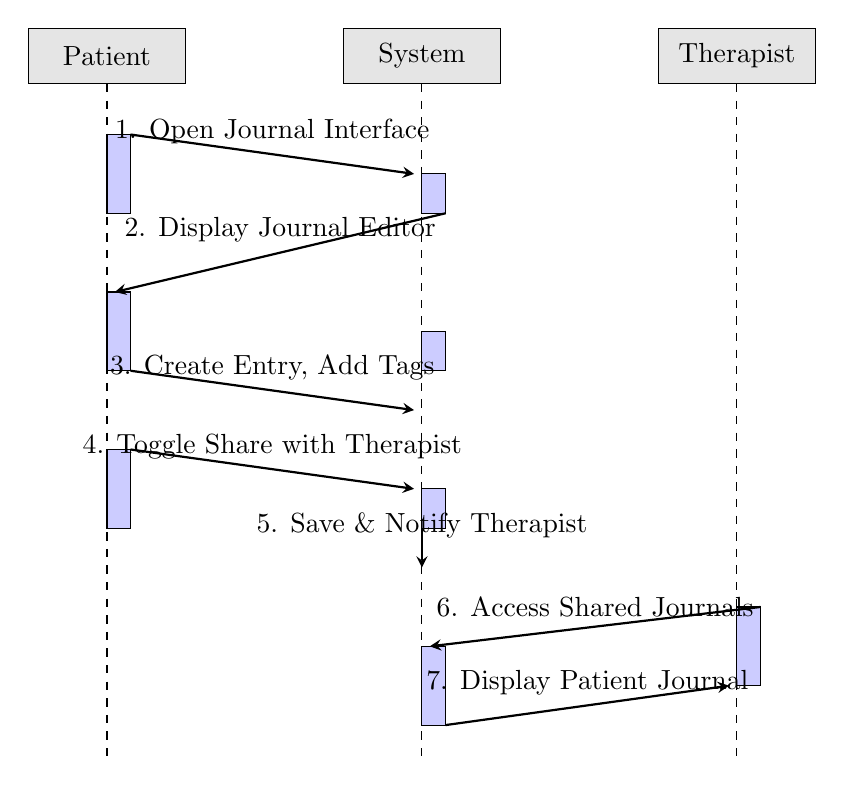
\begin{tikzpicture}
\tikzstyle{actor}=[draw, rectangle, minimum width=2cm, minimum height=0.7cm, fill=gray!20, text centered]
\tikzstyle{line}=[draw, -stealth, thick]
\tikzstyle{lifeline}=[draw, dashed]
\tikzstyle{activation}=[draw, fill=blue!20, minimum width=0.3cm]

% Define actors
\node[actor] (patient) at (0,0) {Patient};
\node[actor] (system) at (4,0) {System};
\node[actor] (therapist) at (8,0) {Therapist};

% Draw lifelines
\draw[lifeline] (patient) -- +(0,-9);
\draw[lifeline] (system) -- +(0,-9);
\draw[lifeline] (therapist) -- +(0,-9);

% Activation boxes
\draw[activation] (0,-1) rectangle +(0.3,-1);
\draw[activation] (4,-1.5) rectangle +(0.3,-0.5);
\draw[activation] (0,-3) rectangle +(0.3,-1);
\draw[activation] (4,-3.5) rectangle +(0.3,-0.5);
\draw[activation] (0,-5) rectangle +(0.3,-1);
\draw[activation] (4,-5.5) rectangle +(0.3,-0.5);
\draw[activation] (8,-7) rectangle +(0.3,-1);
\draw[activation] (4,-7.5) rectangle +(0.3,-1);

% Message flow
\draw[line] (0.3,-1) -- node[above] {1. Open Journal Interface} (3.9,-1.5);
\draw[line] (4.3,-2) -- node[above] {2. Display Journal Editor} (0.1,-3);
\draw[line] (0.3,-4) -- node[above] {3. Create Entry, Add Tags} (3.9,-4.5);
\draw[line] (0.3,-5) -- node[above] {4. Toggle Share with Therapist} (3.9,-5.5);
\draw[line] (4,-6) -- node[above] {5. Save \& Notify Therapist} (4,-6.5);
\draw[line] (8.3,-7) -- node[above] {6. Access Shared Journals} (4.1,-7.5);
\draw[line] (4.3,-8.5) -- node[above] {7. Display Patient Journal} (7.9,-8);
\end{tikzpicture}
\caption{Sequence Diagram: Journal Entry Process}
\end{figure}

\subsubsection{Use Case Description}
\begin{table}[h]
\centering
\begin{tabular}{|p{3cm}|p{10cm}|}
\hline
\textbf{Use Case} & Journal Entries \\
\hline
\textbf{Actor} & Patient, Therapist \\
\hline
\textbf{Precondition} & 
\begin{itemize}
    \item Patient has an active account
    \item Journaling feature is enabled
    \item Patient has authenticated successfully
\end{itemize} \\
\hline
\textbf{Main Scenario Description} & 
\begin{enumerate}
    \item Patient accesses the journal section in the application
    \item System presents journal entry editor with text formatting options
    \item Patient creates a new entry with title, content, and optional tags
    \item Patient may choose to make entry private or shared with therapist
    \item System saves the entry with timestamp and sharing preferences
    \item If shared, therapist receives notification of new journal entry
    \item Therapist can view shared entries during session preparation
    \item Patient can edit or delete their journal entries at any time
\end{enumerate} \\
\hline
\textbf{Postcondition} & 
\begin{itemize}
    \item Journal entry is stored in the system
    \item Entry is accessible to patient and (if shared) to therapist
    \item Entries are available for reference during therapy sessions
\end{itemize} \\
\hline
\textbf{Exception} & 
\begin{itemize}
    \item If content contains concerning keywords (self-harm, suicide), system may prompt user with crisis resources
    \item If network connection is lost during saving, entry is stored locally until connectivity is restored
    \item If patient attempts to delete a journal entry already reviewed by therapist, system prompts for confirmation
\end{itemize} \\
\hline
\end{tabular}
\caption{Use Case Description: Journal Entries}
\end{table}

\subsection{Use Case 6: Chatbot Assistance}
\begin{figure}[h]
\centering
\begin{tikzpicture}
\tikzstyle{actor}=[draw, rounded corners=3pt, fill=gray!20, text width=2cm, minimum height=1cm, align=center]
\tikzstyle{usecase}=[draw, ellipse, fill=blue!20, text width=3.5cm, align=center]
\tikzstyle{system}=[draw, rectangle, dashed, minimum width=12cm, minimum height=8cm]
\tikzstyle{line}=[draw]
\tikzstyle{extend}=[draw, ->, >=stealth, dashed]

% System boundary
\node[system] (sys) at (4,0) {};
\node[align=center] at (4,4) {\textbf{MindCare-IA: Chatbot Assistance}};

% Actors
\node[actor] (patient) at (-2,0) {Patient};
\node[actor] (system) at (10,0) {AI System};

% Use Cases
\node[usecase] (start) at (2,2) {Start Conversation};
\node[usecase] (askQuestions) at (2,0) {Ask Mental Health Questions};
\node[usecase] (coping) at (2,-2) {Get Coping Strategies};
\node[usecase] (process) at (6,1) {Process Natural Language};
\node[usecase] (generate) at (6,-1) {Generate Therapeutic Response};

% Connections
\draw[line] (patient) -- (start);
\draw[line] (patient) -- (askQuestions);
\draw[line] (patient) -- (coping);
\draw[line] (system) -- (process);
\draw[line] (system) -- (generate);
\draw[extend] (askQuestions) -- (process) node[midway, above, sloped, font=\small] {<<includes>>};
\draw[extend] (process) -- (generate) node[midway, above, sloped, font=\small] {<<includes>>};
\draw[extend] (generate) -- (coping) node[midway, above, sloped, font=\small] {<<extends>>};
\end{tikzpicture}
\caption{Use Case Diagram: Chatbot Assistance}
\end{figure}

\subsubsection{Sequence Diagram for Chatbot Assistance}
\begin{figure}[h]
\centering
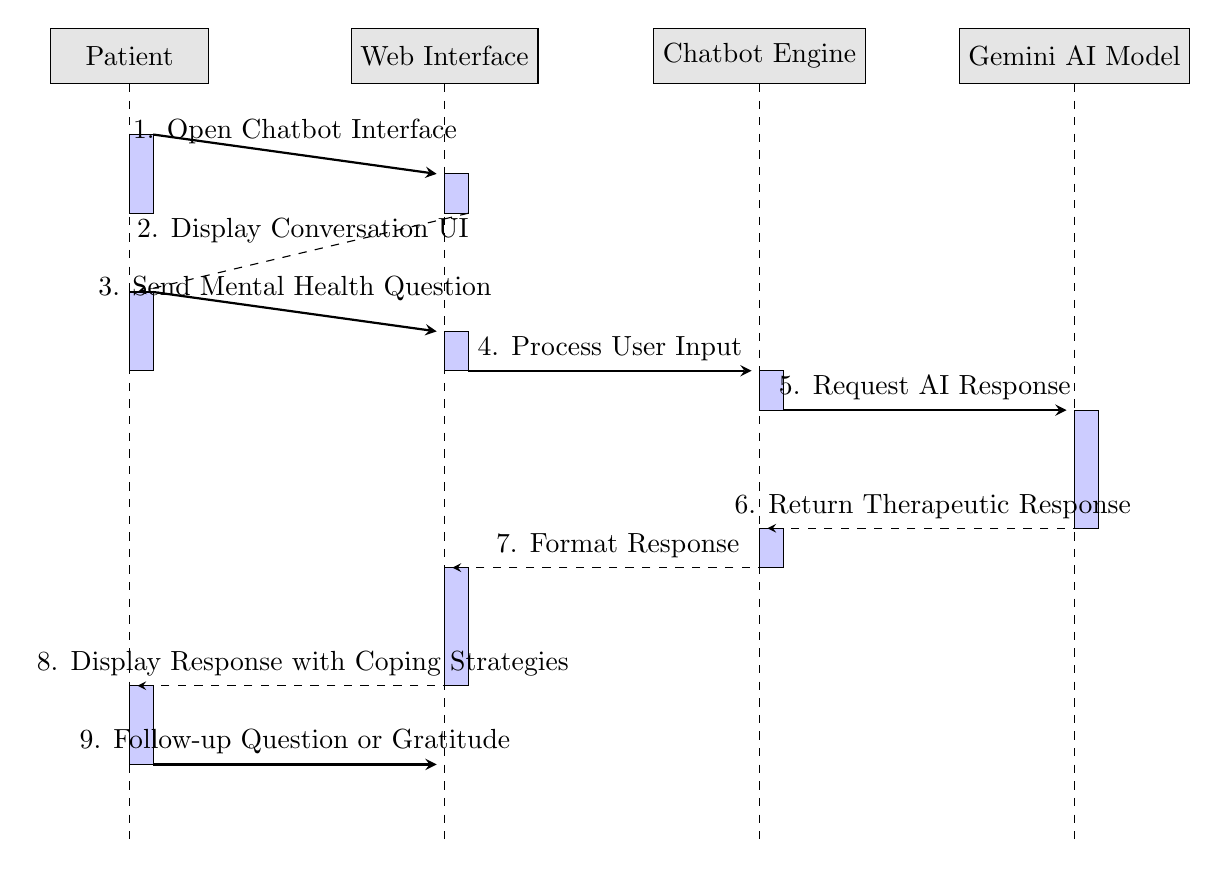
\begin{tikzpicture}
\tikzstyle{actor}=[draw, rectangle, minimum width=2cm, minimum height=0.7cm, fill=gray!20, text centered]
\tikzstyle{line}=[draw, -stealth, thick]
\tikzstyle{return}=[draw, -stealth, dashed]
\tikzstyle{lifeline}=[draw, dashed]
\tikzstyle{activation}=[draw, fill=blue!20, minimum width=0.3cm]

% Define actors
\node[actor] (patient) at (0,0) {Patient};
\node[actor] (ui) at (4,0) {Web Interface};
\node[actor] (chatbot) at (8,0) {Chatbot Engine};
\node[actor] (ai) at (12,0) {Gemini AI Model};

% Draw lifelines
\draw[lifeline] (patient) -- +(0,-10);
\draw[lifeline] (ui) -- +(0,-10);
\draw[lifeline] (chatbot) -- +(0,-10);
\draw[lifeline] (ai) -- +(0,-10);

% Activation boxes
\draw[activation] (0,-1) rectangle +(0.3,-1);
\draw[activation] (4,-1.5) rectangle +(0.3,-0.5);
\draw[activation] (0,-3) rectangle +(0.3,-1);
\draw[activation] (4,-3.5) rectangle +(0.3,-0.5);
\draw[activation] (8,-4) rectangle +(0.3,-0.5);
\draw[activation] (12,-4.5) rectangle +(0.3,-1.5);
\draw[activation] (8,-6) rectangle +(0.3,-0.5);
\draw[activation] (4,-6.5) rectangle +(0.3,-1.5);
\draw[activation] (0,-8) rectangle +(0.3,-1);

% Message flow
\draw[line] (0.3,-1) -- node[above] {1. Open Chatbot Interface} (3.9,-1.5);
\draw[return] (4.3,-2) -- node[above] {2. Display Conversation UI} (0.1,-3);
\draw[line] (0.3,-3) -- node[above] {3. Send Mental Health Question} (3.9,-3.5);
\draw[line] (4.3,-4) -- node[above] {4. Process User Input} (7.9,-4);
\draw[line] (8.3,-4.5) -- node[above] {5. Request AI Response} (11.9,-4.5);
\draw[return] (12.3,-6) -- node[above] {6. Return Therapeutic Response} (8.1,-6);
\draw[return] (8.3,-6.5) -- node[above] {7. Format Response} (4.1,-6.5);
\draw[return] (4.3,-8) -- node[above] {8. Display Response with Coping Strategies} (0.1,-8);
\draw[line] (0.3,-9) -- node[above] {9. Follow-up Question or Gratitude} (3.9,-9);
\end{tikzpicture}
\caption{Sequence Diagram: Chatbot Assistance Interaction}
\end{figure}

\subsubsection{Use Case Description}
\begin{table}[h]
\centering
\begin{tabular}{|p{3cm}|p{10cm}|}
\hline
\textbf{Use Case} & Chatbot Assistance \\
\hline
\textbf{Actor} & Patient, AI System \\
\hline
\textbf{Precondition} & 
\begin{itemize}
    \item Patient has an active account
    \item Patient has authenticated successfully
    \item Chatbot service is operational
    \item AI model is available for inference
\end{itemize} \\
\hline
\textbf{Main Scenario Description} & 
\begin{enumerate}
    \item Patient navigates to chatbot interface within the application
    \item System initializes conversation with a welcoming prompt
    \item Patient types a mental health question or concern
    \item System processes natural language input
    \item Chatbot analyzes message context and conversation history
    \item AI generates an empathetic, therapeutically-informed response
    \item Response includes validation, support, and applicable coping strategies
    \item Patient may continue conversation with follow-up questions
    \item System maintains context throughout the conversation session
    \item Conversation history is saved for patient reference
\end{enumerate} \\
\hline
\textbf{Postcondition} & 
\begin{itemize}
    \item Patient receives supportive guidance in real-time
    \item Conversation is stored securely in patient's account
    \item Interaction data improves future chatbot responses
    \item Patient has access to suggested coping strategies
\end{itemize} \\
\hline
\textbf{Exception} & 
\begin{itemize}
    \item If patient expresses crisis or suicidal ideation, chatbot provides crisis resources and encourages professional help
    \item If AI cannot understand the query, system requests clarification
    \item If connectivity issues occur, system notifies patient and suggests reconnecting
    \item If inappropriate content is detected, system provides a neutral redirection
    \item If technical failure occurs, system offers alternative support channels
\end{itemize} \\
\hline
\end{tabular}
\caption{Use Case Description: Chatbot Assistance}
\end{table}

\subsection{Use Case 7: Therapist Verification}
\begin{figure}[h]
\centering
\begin{tikzpicture}
\tikzstyle{actor}=[draw, rounded corners, fill=gray!20, text width=2cm, minimum height=1cm, align=center]
\tikzstyle{usecase}=[draw, ellipse, fill=blue!20, text width=3.5cm, align=center]
\tikzstyle{system}=[draw, rectangle, dashed, minimum width=12cm, minimum height=8cm]

% System boundary
\node[system] (sys) at (4,0) {};
\node[align=center] at (4,4) {MindCare-IA: Therapist Verification};

% Actors
\node[actor] (therapist) at (-2,0) {Therapist};
\node[actor] (admin) at (10,0) {System Administrator};

% Use Cases
\node[usecase] (submit) at (2,2) {Submit Credentials};
\node[usecase] (upload) at (2,-1) {Upload Documents};
\node[usecase] (review) at (6,2) {Review Application};
\node[usecase] (verify) at (6,-1) {Verify License};
\node[usecase] (approve) at (4,0.5) {Approve/Reject};

% Connections
\draw (therapist) -- (submit);
\draw (therapist) -- (upload);
\draw (admin) -- (review);
\draw (admin) -- (verify);
\draw (admin) -- (approve);
\draw[dashed, ->] (submit) -- (review);
\draw[dashed, ->] (upload) -- (verify);
\end{tikzpicture}
\caption{Use Case Diagram: Therapist Verification}
\end{figure}

\textbf{Description:} This use case outlines the process for validating therapist credentials to ensure platform integrity and patient safety.

\textbf{Primary Actors:} Therapist, System Administrator

\textbf{Preconditions:}
\begin{itemize}
    \item Therapist has registered with professional details
    \item Required verification documents are available
\end{itemize}

\textbf{Main Flow:}
\begin{enumerate}
    \item Therapist submits license information and uploads verification documents
    \item System securely stores documents and creates verification case
    \item Administrator reviews submitted credentials and documentation
    \item Administrator validates license information against official databases
    \item Administrator approves or rejects verification
    \item System updates therapist profile status accordingly
\end{enumerate}

\textbf{Alternative Flows:}
\begin{itemize}
    \item If documentation is incomplete, system requests additional information
    \item If verification fails, administrator provides reason and therapist may resubmit
    \item If license expires, system flags profile for re-verification
\end{itemize}

\textbf{Postconditions:} Therapist receives verified status allowing patient interaction, or is notified of rejection with reason